\section*{Related Work}
\subsection{Related Work}
    \begin{frame}
       \begin{columns}
            \column{0.5\textwidth}
                Platforms for reusing of tools
                \begin{itemize}
                    \item Moose
                    \item RepoGrams
                    \item Kenyon and Sourcerer
                    \item Alitheia Core
                    \item FLOSSMole
                    \item Groundhog
                \end{itemize}

            \column{0.5\textwidth}
                Provides a repository of datasets
                \begin{itemize}
                    \item GHTorrent
                    \item Promise Repository
                    \item SourcererDB
                    \item Boa
                \end{itemize}
        \end{columns}
    \end{frame}

\section{Summary}
    \subsection{Summary}
        \begin{frame}
            \begin{figure}
                \centering
                    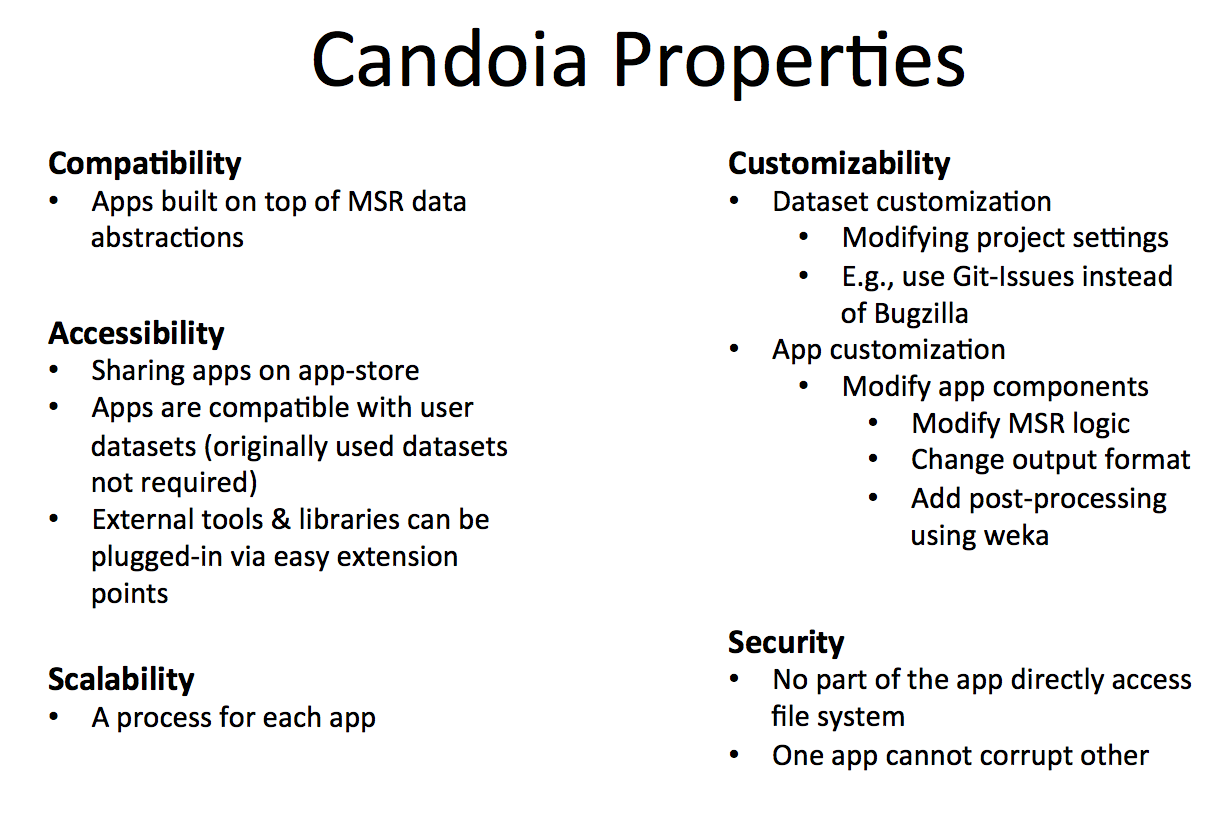
\includegraphics[scale=0.2]{figures/summary.png}
            \end{figure}
        \end{frame}


\makeatletter % to change template
    \setbeamertemplate{headline}[default] % not mandatory, but I though it was better to set it blank
    \def\beamer@entrycode{\vspace*{-\headheight}} % here is the part we are interested in :)
\makeatother

        \begin{frame}
                \begin{figure}
                    \centering
                    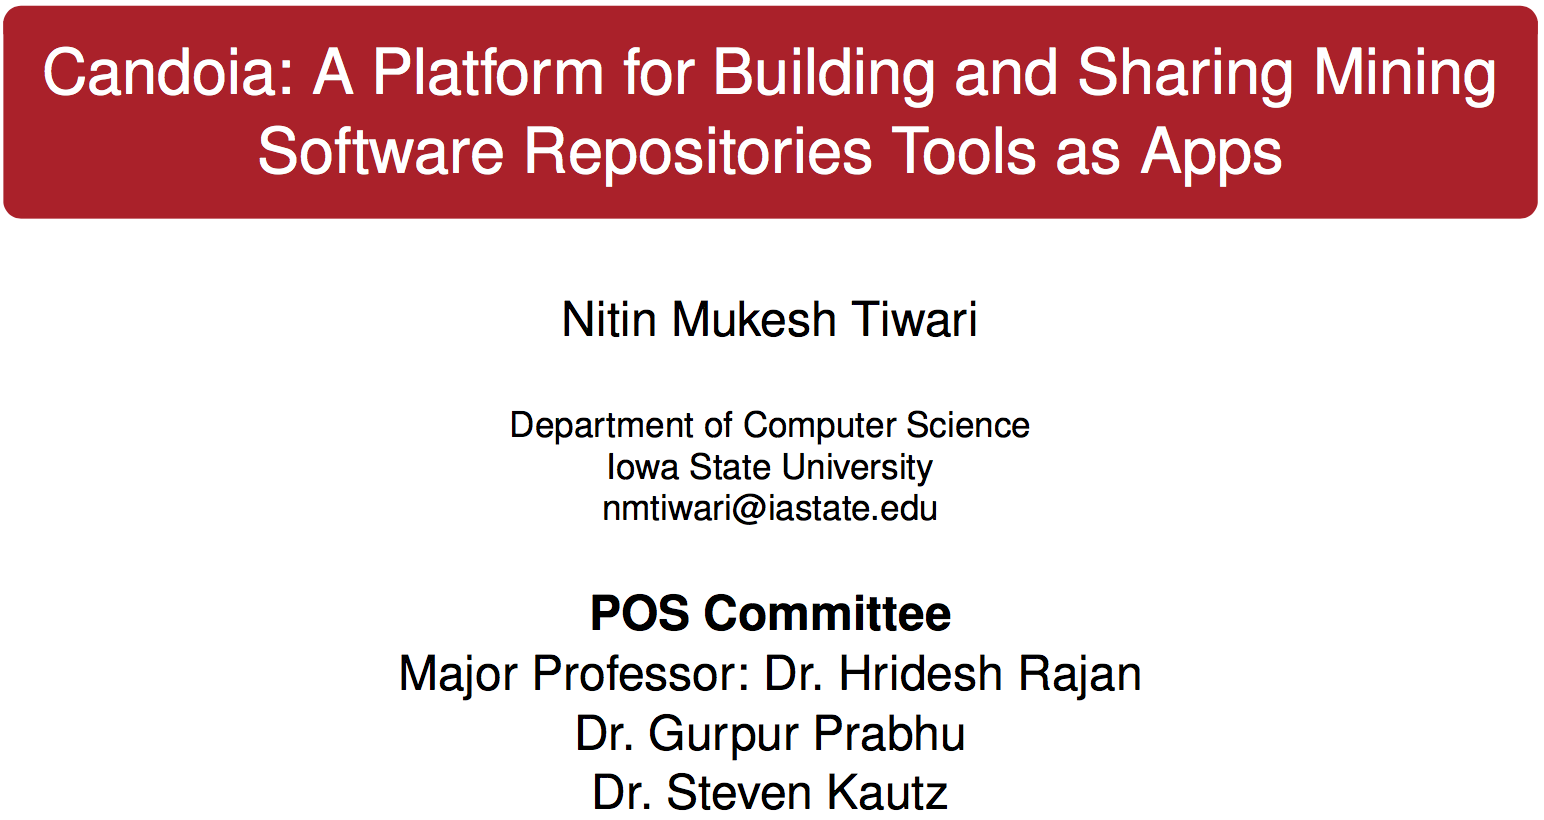
\includegraphics[scale=0.2]{figures/thankyou.png}

                \end{figure}
        \end{frame}


